\documentclass{article}
\usepackage{polski}
\usepackage[utf8]{inputenc}
\usepackage{tikz}
\usetikzlibrary{matrix}
\usepackage[a4paper, total={6in, 8in}]{geometry}
\usepackage{caption}
\usepackage{graphicx}
\usepackage{float}
\usepackage{url}
\usepackage{minted}

\newcommand*{\GridSize}{4}

\newcommand*{\ColorCells}[1]{% #1 = list of x/y/color
  \foreach \x/\y/\color in {#1} {
    \node [fill=\color, draw=none, thick, minimum size=1.5cm]
      at (\x-.5,\GridSize+0.5-\y) {};
    }%
}%


\title{Rozwiązywanie łamigłówki Kuromasu algorytmem genetycznym}
\author{Sebastian Rychert}
\date{April 2022}

\begin{document}

\maketitle

\tableofcontents
\clearpage

\section{Temat pracy}
Niniejsza praca skupia się na przedstawieniu sposobu rozwiązania zagadki Kuromasu za pomocą algorytmy genetycznego oraz porównaniu wyników w zależności od stopnia skomplikowania łamigłówki. Najważniejsze kryteria to skuteczność algorytmu oraz czas potrzebny na znalezienie rozwiązania. Praca zawiera wstawki kodu źródłowego z języka python w wersji 3.8. Wykorzystano bibliotekę PyGAD.

\section{Opis gry}
\subsection{Zasady}
W Kuromasu gra się na prostokątnej siatce. Na początku wszystkie komórki są białe, a niektóre mają w sobie liczby. Celem gry jest określenie koloru każdej komórki (biała lub czarna).\\
\newline
Poniższe zasady określają sposób wyboru koloru dla każdej komórki:

\begin{itemize}
  \item Każda liczba na planszy reprezentuje liczbę białych komórek, które można zobaczyć z tej komórki, łącznie z nią. Komórkę można zobaczyć z innej komórki, jeśli obie komórki znajdują się w tym samym wierszu lub kolumnie i nie ma między nimi czarnych komórek w tym wierszu lub kolumnie.
  \item Ponumerowane komórki nie mogą być czarne.
  \item Żadne dwie czarne komórki nie mogą przylegać do siebie w pionie lub poziomie.
  \item Wszystkie białe komórki muszą być połączone poziomo lub pionowo.
\end{itemize}

\subsection{Przykład rozwiązania}
\vspace{1cm}


\begin{center}
    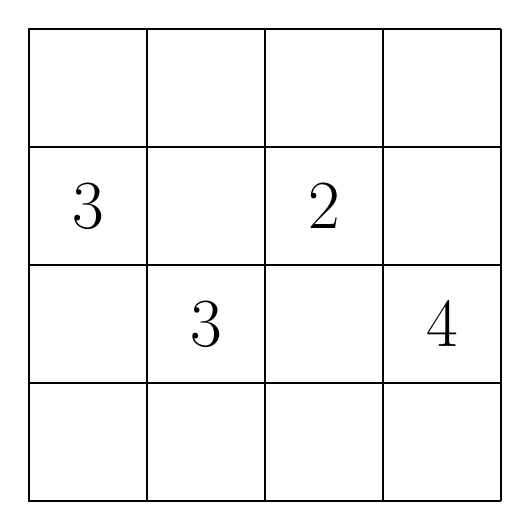
\begin{tikzpicture}[scale=1.5]
        \begin{scope}[thick,local bounding box=name]
            \Huge
            \ColorCells{}
            \node[matrix of math nodes,anchor=south west,inner sep=0pt,xshift=-\pgflinewidth,yshift=-\pgflinewidth,
            nodes={draw,minimum size=1.5cm,anchor=center},
            column sep=-\pgflinewidth,row sep=-\pgflinewidth]
            {\; &  &  &  \\
            3 &  & 2 &  \\
            & 3 &  & 4 \\
            \; &  &  &  \\};
            \draw (0, 0) grid (\GridSize, \GridSize);
        \end{scope}
    \end{tikzpicture}
\end{center}

\vspace{1cm}

\begin{center}
    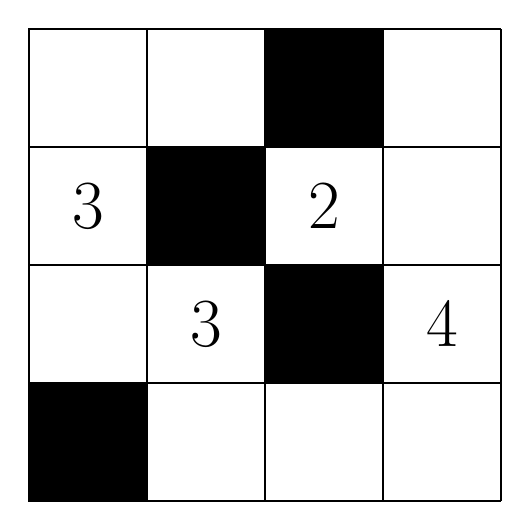
\begin{tikzpicture}[scale=1.5]
        \begin{scope}[thick,local bounding box=name]
            \Huge
            \ColorCells{3/1/black, 2/2/black, 3/3/black, 1/4/black}
            \node[matrix of math nodes,anchor=south west,inner sep=0pt,                  xshift=-\pgflinewidth,yshift=-\pgflinewidth,
            nodes={draw,minimum size=1.5cm,anchor=center},
            column sep=-\pgflinewidth,row sep=-\pgflinewidth]
            {\; &  &  &  \\
            3 &  & 2 &  \\
            & 3 &  & 4 \\
            \; &  &  &  \\};
            \draw (0, 0) grid (\GridSize, \GridSize);
        \end{scope}
    \end{tikzpicture}
    \label{Rozwiązany}

\end{center}

\section{Algorytm}

\renewcommand{\theFancyVerbLine}{
  \sffamily\textcolor[rgb]{0.5,0.5,0.5}{\scriptsize\arabic{FancyVerbLine}}}

\subsection{Reprezentacja planszy}
Plansza w programie jest reprezentowana jako dwuwymiarowa tablica numpy. Dane potrzebne do jej utworzenia czytane są z pliku "puzzles.json" pod konkrentynm kluczem np. "0". Puste pola są zerami.

\begin{minted}[mathescape, linenos, numbersep=5pt, gobble=2, frame=lines, framesep=2mm]{python}
    # load puzzles from file
    puzzles = {}
    with open("puzzles.json", "r") as f:
        puzzles = json.load(f)

    # make a board for puzzle - args.p is puzzle id flag e.g. "0"
    board = np.array(puzzles[args.p])
\end{minted}

\subsection{Parametry}
Aby uruchomić algorytm genetyczny musimy zdefiniowac szereg parametrów.\\
\newline
Pierwszym z nich jest \textit{\textbf{gene\_space}}, który określa możliwe geny do wygenerowania w rozwązaniu. Nasz algorytm będzie generował liczby binarne, to znaczy 0 lub 1.\\
\newline
Następnie ustawiamy \textit{\textbf{num\_genes}}, odpowiadający za długość chromosomu. Wartość taka jak liczba pustych pól w łamigłówce.\\
\newline
Kolejnym ważnym parameterm jest \textit{\textbf{sol\_per\_pop}}, odpowiadający za wielkość populacji, czyli inaczej liczbę chromosomów w danej generacji.\\
\clearpage
Trzy kolejne parametry są ustawiane jako mały procent wielkości populacji.\\
\textit{\textbf{num\_generations}} \hspace{0.5cm} - Liczba generacji\\
\textit{\textbf{num\_parents\_mating}} - Ile wybrać rodziców do rozmnażania\\
\textit{\textbf{keep\_parents}} \hspace{1.3cm} - Ile rodziców zachować\\
\newline
Określimy także punkt zatrzymania algorytmu w przypadku braku postępów przez znaczną część pokoleń -
\textit{\textbf{saturate}} - oraz procent szansy na mutacje \textit{\textbf{mutation\_percent\_genes}}

\begin{minted}[mathescape, linenos, numbersep=5pt, gobble=2, frame=lines, framesep=2mm]{python}
    gene_space = [1, 0]

    # calc gene length from board
    num_genes = 0
    for i in board.flatten():
        if i == 0:
            num_genes += 1

    # population size
    sol_per_pop = board.shape[0] * board.shape[1] * 10
    num_generations = int(2 * sol_per_pop)
    num_parents_mating = int(0.25 * sol_per_pop)
    keep_parents = int(0.01 * sol_per_pop)
    s = int(0.02 * num_generations)
    saturate = "saturate_{s}".format(s=15 if s < 15 else s)

    # sss = steady, rws=roulette, rank = rankingowa, tournament = turniejowa
    parent_selection_type = "sss"
    crossover_type = "single_point"
    mutation_type = "random"
    # small boards - smaller mutation percent and bigger for bigger boards
    mutation_percent_genes = 120 / num_genes if num_genes <= 50 else 100 * (2 / num_genes)
\end{minted}

\subsection{Funkcja przystosowania – (ang. fitness function)}
Jest to główny element algorytmu który musimy zdefiniować. Na podstawie wyniku funkcji ewaluujemy poprawność rozwiązania dla każdego chromosomu. Celem algorytmu jest osiągnięcie wartości 0. Punkty ujemne przydzielamy w liczbie:\\

\begin{itemize}
  \item Wynik z absolutnej różnicy wartości każdej ponumerowanej komórki z liczbą komórek, które widzi w pionie i poziomie.
  \item 2 punkty za każdą parę czarnych komórek (para - 2 komórki sąsiadujące w pionie lub poziomie)
  \item Potęga o podstawie równej 2 oraz wykładniku będącym liczbą wysp, czyli odseparownaych od reszty skupisk białych komórek, pomniejszony o 1. Wynik potęgowania zmniejszamy o 1 ($2^1 - 1 = 0$)
\end{itemize}


\begin{minted}[mathescape, linenos, numbersep=5pt, gobble=2, frame=lines, framesep=2mm]{python}

    def fitness_func(solution, solution_idx):
        # board for solution
        board_s = makeBoardWithSoution(solution)
        points = 0
        # deep first search object
        dfs = DFS()
        # find starting point for dfs
        firstA = np.argwhere(board_s != 1)[0]
        first = (firstA[0], firstA[1])

        # calculate points
        for idx, x in np.ndenumerate(board_s):
            points -= whiteCellsPoints(x, idx, board_s)
            points -= blackCellsPoints(x, idx, board_s)

        # check if there is only one island else give punishment points
        islands = dfs.getNumberOfIslands(board_s, first)
        points -= 2 ** (islands - 1) - 1

    return points
\end{minted}

\section{Wyniki}

\subsection{Sposób pomiaru}
Algorytm został uruchomiony na 10 różnych łamigłówkach o rosnącym stopniu trudności; zaczynając na planszy o wymiarach 4x4, a kończąc na 11x11. Każda plansza była poddana próbie rozwiązania 10 razy. Dla każdej planszy zapisany został procent sukcesu, średni czas rozwiązania oraz średni numer generacji rozwiązania. Próby zakończone porażką, to znaczy wartością fitness różną od 0, zostały pominięte.\\
\newline
Aby zwiększyć predkość przeprowadzania testów została użyta technika przetwarzania wieloprocesorowego.

\begin{minted}[mathescape, linenos, numbersep=5pt, gobble=2, frame=lines, framesep=2mm]{python}
    results = []
    with concurrent.futures.ProcessPoolExecutor() as executor:
        # make list of len = runs
        l = list(range(0, runs))
        # run the algorithm for the number of processes equal to "runs"
        pool = executor.map(runGA, l)
        for res in pool:
            results.append(res)
\end{minted}

\subsection{Tabela}

% Please add the following required packages to your document preamble:
% \usepackage{graphicx}
\begin{table}[H]
\centering
\caption{Wyniki testów}
\resizebox{\textwidth}{!}{%
\begin{tabular}{cccccc}
\multicolumn{1}{l}{} & \multicolumn{1}{l}{rozmiar} & \begin{tabular}[c]{@{}c@{}}długość\\ chromosomu\end{tabular} & \begin{tabular}[c]{@{}c@{}}procent\\ sukcesu\end{tabular} & \begin{tabular}[c]{@{}c@{}}średni czas\\ sukcesu {[}s{]}\end{tabular} & \begin{tabular}[c]{@{}c@{}}średnia generacja\\ sukcesu\end{tabular} \\
puzzle               &                             &                                                              &                                                           &                                                                       &                                                                     \\
0                    & 4x4                         & 12                                                           & 100\%                                                     & 0.179                                                                 & 65                                                                  \\
1                    & 5x5                         & 19                                                           & 100\%                                                     & 1.004                                                                 & 111                                                                 \\
2                    & 7x6                         & 32                                                           & 100\%                                                     & 3.535                                                                 & 191                                                                 \\
3                    & 7x7                         & 40                                                           & 70\%                                                      & 5.218                                                                 & 184                                                                 \\
4                    & 8x7                         & 42                                                           & 100\%                                                     & 6.712                                                                 & 171                                                                 \\
5                    & 8x7                         & 46                                                           & 80\%                                                      & 9.900                                                                 & 311                                                                 \\
6                    & 9x9                         & 59                                                           & 70\%                                                      & 53.922                                                                & 307                                                                 \\
7                    & 9x9                         & 64                                                           & 20\%                                                      & 69.261                                                                & 609                                                                 \\
8                    & 9x9                         & 71                                                           & 10\%                                                      & 50.431                                                                & 8                                                                   \\
9                    & 11x11                       & 101                                                          & 0\%                                                       & -                                                                     & -
\end{tabular}%
}
\end{table}

\subsection{Wykresy}

\begin{center}
  \makebox[\textwidth]{\includegraphics[width=\linewidth]{line-graph-sukces.png}}
  \makebox[\textwidth]{\includegraphics[width=\linewidth]{line-graph-czas.png}}
\end{center}

\subsection{Podsumowanie}
Przeprowadzone testy wskazują iż algorytm znajduje rozwiązanie w mniejszych oraz średnich planszach, ale nie radzi sobie już z większymi planszami. Punktem diametralnego spadku procentu sukcesu wydaje się być długość chromosomu równa 60. Algorytm powyżej tej długości o wiele częściej wpada w minima lokalne, które nie pasują ostatecznie do prawidłowego rozwiązania.\\
Wyniki planszy o id "8" sugerują, iż jedynie początkowa "szczęśliwa" kombinacja jest wstanie doprowadzić do rozwiązania na większej planszy - świadczy o tym bardzo mała liczba generacji równa 8.

\begin{thebibliography}{9}
\bibitem{link_latlng_00} Wikipedia strona Kuromasu \url{https://en.wikipedia.org/wiki/Kuromasu}
\bibitem{link_latlng_00} PyGad Dokumentacja  \url{https://pygad.readthedocs.io/en/latest/}
\bibitem{link_latlng_00} Katalog łamigłówek \url{https://www.math.edu.pl/kuromasu}
\end{thebibliography}

\end{document}
